\chapter{Úvod}
Koža je najväčší orgán ľudského teľa, ktorý pokrýva telo človeka. Kvôli tomu je prirodzené, že podlieha rôznym chorobám a je náchylná na početné zranenia. Medzi časté zranenia patria aj kožné rany, ktoré sú spôsobené rôznymi faktormi anatomického a fyziologického charakteru, či už sa jedná vnútorne príčiny, alebo vonkajšie. Rany môžu byť od tých menej vážnych, až po tie najvážnejšie. Menej vážne rany zasahujú väčšinou do pokožky, zamše a podkožného tuku. Avšak vážnejšie rany už môžu zasahovať aj nervovo-cievnych zväzkov a orgánov, a tým tak významne ohrozovať život postihnutého pacienta. Jedno z najvýznamnejších delení rán je delenie podľa priebehu. Takéto delenie rozdeľuje rany na, rany akútne a rany chronické. Akútne rany vznikajú v zdravom kožnom tkanive, hoja sa v krátkom čase a bez komplikácií. S takýmito ranami sa človek stretá často vo svojom živote, či už pri porezaní kože, odretí kože, alebo iných bežných vonkajších kožných poraneniach. Chronické rany, ktoré sú stredobodom tejto práce, na druhú stranu trvajú dlhšie než 4 týždne, a aj napriek všetkej odpovedajúcej liečbe nevykazujú tendenciu hojenia. Za najbežnejšiu príčinu takýchto rán sa považujú lokálne poruchy výživy kože, pôsobenie tlaku, alebo systémové ochorenie. 

Táto diplomová práca vznikla z dôvodu neexistencie nástroja, ktorý by pomohol lekárom a zdravotným sestrám so sledovaním chronických rán, ich priebehu a vývoja v čase. Pomocou aplikácie by malo byť možné detekovať, lokalizovať a určiť plochu chronickej rany. Zároveň by malo byť možné porovnávať jednotlivé výsledky danej rany v histórií a tak adekvátne reagovať na danú situáciu zmenou liečby, poprípade zavedením opatrení proti zhoršovaniu diagnózy. V momentálnej situácií určenie plochy chronickej rany prebieha zdravotnými sestrami za pomoci pravítok a iných merných pomôcok. Táto klasická metóda získavania informácií o rane a zisťovania plochy nie je veľmi efektívna a ani presná, kedže rany môžu mať rôzne tvary a podoby.
	
Nasledujúca kapitola sa venuje teoretickému rozboru a obsahuje informácie potrebné k základnému pochopeniu problematiky chronických rán. Hneď po tom nasleduje kapitola, ktorá rozoberá technológie, ktoré boli potrebné pri vývoji aplikácie a jej súčastí. Ďalšia kapitola sa venuje analýze a návrhu samotnej mobilne aplikácie a jej serverových súčastí. Konkrétne popisuje návrh grafického užívateľského rozhrania, ale aj návrh aplikačného rozhrania REST a výber vhodných technologických prostriedkov.

\chapter{Teoretický rozbor}
Táto kapitola sa zaoberá teoretickým rozborom problematiky chronických rán, ktoré sú jadrom tejto práce. Kapitola sa snaží najprv vysvetliť základné pojmy a termíny týkajúce sa problematiky a následne vysvetľuje samotné chronické rany, ich príčiny vzniku a prejavy. Celá kapitola vychádza z informácií dostupných na webovej stránke \cite{pcCdSrbbhhlr5YcQ} a z kníh \cite{Hlinkova2015} a \cite{Pokorna2012}.  

\section{Koža}
Koža je najväčší orgán ľudského tela, ktorý má u dospelého človeka veľkosť plochy od 1,6 až do 1,8 metra štvorcového a váži približne 7 percent celkovej telesnej hmotnosti. Hrúbka kože sa pohybuje od 0,4 až po 4 milimetre a líši sa podľa jednotlivých častí tela. Najtenšia je na očných viečkach, najhrubšia zase na chrbte.

Kože nielenže plní funkciu obalu človeka, ale okrem toho plní aj celú radu pre človeka oveľa dôležitejších funkcií, medzi ktoré patrí:
\begin{itemize}  
\item \textbf{ochrana -} pred vstupom nečistôt do organizmu, pred stratou tekutín, proti teplotným výkyvom
\item \textbf{vnímanie -} zmyslové buky v koži informujú o teplote alebo poranení
\item \textbf{termoregulácia -} tepelná izolácia, výmena tepla medzi organizmom a okolím
\item \textbf{skladovanie -} koža sa podiela na látkovej výmene a uchovávaní tukov, vody, minerálnych látok a vitamínov
\item \textbf{vylučovanie -} mazové a potné žľazy vylučujú vodu, soli, tuky, oxid uhličitý a dusíkaté látky.
\item \textbf{vstrebávanie -} kožou prenikajú látky rozpustné v tukoch a dýchacie plyny
\item \textbf{estetická funkcia -} vzhľad a úprava kože je jedným z prvých znakov, ktorých si ľudia pri vzájomnom kontakte všímajú
\end{itemize}

Kôža je zložená z 3 hlavných časti, a to z pokožky (epidermis), zamši (dermis) a podkožia (subcutis). Tieto 3 hlavné vrstvy je možné vidieť na obrázku dole. Okrem týchto hlavných vrstiev sa skladá aj z vlasov/chlpov, nechtov a žliaz (mazové, potné, pachové a mliečne). Dokopy sa nazývajú kožné deriváty. 
\begin{itemize}  
\item \textbf{Pokožka -} vonkajšia vrstva. Je tvorená niekoľkými vrstvami kožných buniek. V spodných častiach pokožky sa bunky neustále delia a vytláčajú bunky nad sebou bližšie k povrchu. Postupom do horných vrstiev pokožky bunky postupne rohovatejú, odumierajú a odlupujú sa. Pomocou tohoto procesu dochádza k plynulej obmene celej pokožky. Z človeka sa počas jeho života odlúpne v priemere asi 20 kilogramov mŕtvych buniek. 
\item \textbf{Zamša -} stredná vrstva. Je tvorená väzivom, sieťou ciev a nervových zakončení. Táto vrstva rozhoduje o pevnosti kože, jej pružnosti a mechanickej odolnosti. Medzi dôležité súčasti zamše patria hlavne nervové zakončenia, vďaka ktorým vnímame teplo, chlad a bolesť. Jemné cievy zase slúžia pre reguláciu tepla a imunitné bunky zaisťujú ochranu.
\item \textbf{Podkožie -} najhlbšia vrstva. Je tvorená riedkym väzivom a tukom. Hlavnou úlohou podkožia je ochrana proti teplotným vplyvom a mechanickému poškodeniu. V tukovom tkanive si organizmus uchováva prebytky energie. 
\end{itemize}
\begin{figure}[h]
  \centering
  \includegraphics[scale=0.20]{fig/koza.jpg}
  \caption{Zloženie ľudskej kože. Zdroj \cite{Ebling2016}}
  \label{fig:koza}
\end{figure}

\section{Kožná rana}
Kožná rana je definovaná ako strata, či prerušenie kožného krytu v dôsledku fyzikálneho, mechanického, alebo termického poškodenia, či v dôsledku patofyziologických porúch, alebo akékoľvek poškodenie anatomických, alebo fyziologických funkcií tkaniva.

Kožné rany je možné rozdeliť na jednoduché a komplikované. Jednoduché kožné rany zasahujú do pokožky, zamše a podkožného tuku. Komplikované rany zase narozdiel od jednoduchých prenikajú hlbšie a poškodzujú dôležité nervovo-cievne zväzky a orgány. Komplikované rany je ďalej možné rozdeliť na penetrujúce a nepenetrujúce. Penetrujúca rana preniká do teľnej dutiny. Nepenetrujúca rana naopak nepreniká do telesnej dutiny. U každej rany, či už jednoduchej, komplikovanej, penetrujúcej, alebo nepenetrujúcej určujeme a popisujeme vlastnosti, ktoré sú veľmi dôležité pri sledovaní procesu hojenia rany a voľby optimálnej liečby. Medzi takéto vlastnosti patrí:
\begin{itemize} 
\item lokalizácia rany
\item veľkosť rany
\item hĺbka rany
\item tvar rany
\item smer rany
\item okraje rany
\end{itemize}


\section{Triedenie a typy rán}
Rany a poškodenia je možné deliť do niekoľko skupín podľa rôznych kritérií. Rany sa delia podľa ich priebehu, podľa rozsahu ich poškodenia, podľa množstva choroboplodných zárodkov, podľa spôsobu hojenia, podľa lokalizácie, podľa postihnutých štruktúr a mnoho iných delení, pričom najdôležitejšie delenia sú tie, ktoré sú ďalej popísané podrobnejšie.
Rany podľa priebehu sa delia na:
\begin{itemize} 
\item \textbf{akútne rany -} vznikajú v zdravom kožnom tkanive. Hoja sa obvykle v krátkom čase a bez komplikácií.
\item \textbf{chronické rany -} trvajú dlhšie než 4 týždne, alebo to sú rany, ktoré vznikajú v zmenenom tkanive, a ktoré aj cez všetku odpovedajúcu liečbu nevykazujú známky hojenia.
\end{itemize}
Rany podľa rozsahu sa delia na:
\begin{itemize} 
\item \textbf{uzatvorené rany -} poškodenie bez porušenia integrity kože
\item \textbf{povrchové rany -} poškodenia pokožky
\item \textbf{hlboké rany -} poškodenie až do podkožia
\item \textbf{prenikajúce rany -} zasahujú do teľných dutín
\item \textbf{komplikované rany -} komplexné rozsiahle poranenia s možným poškodením ciev, nervov, svalov, kostí a orgánov
\end{itemize}
Rany podľa množstva choroboplodných zárodkov sa delia na:
\begin{itemize} 
\item \textbf{aseptické rany -} bez zárodkov (chirurgický rez)
\item \textbf{kontaminované rany -} s prítomnosťou zárodkov, ktoré však nemusia vyvolať infekciu
\item \textbf{infikované rany -} s premnoženými mikroorgnizmami (rany vzniknuté po pohryznutí, poprípade zanedbané, alebo zastaralé rany)
\end{itemize}
Rany podľa spôsobu hojenia sa delia na:
\begin{itemize} 
\item \textbf{rany s primárnym hojením -} vďaka zlepeniu/zošitiu okrajov rany nevzniká nové spojivové tkanivo
\item \textbf{rany so sekundárnym hojením -} rana sa hojí novo tvoreným tkanivom
\end{itemize}

\section{Príčiny rán}
Rany môžu vznikať pôsobením rôznych príčin, medzi ktoré patria vonkajšie, vnútorné príčiny alebo kombinácia týchto dvoch. Medzi vonkajšie príčiny patria rany rezné, sečné, tržné, rany spôsobené pohryznutím, bodné, strelné, zhmoždené, popáleniny, omrzliny, poleptaniny a rany spôsobené z ožiarenia. Medzi vnútorné príčiny patria cievne vredy dolných končatín, neuropatické vredy, preležaniny, rany pri nádorových ochoreniach, rany pri infekčných ochoreniach a rany pri imunitných poruchách. Vo všeobecnosti sa dajú príčiny vzniku rán rozdeliť do troch základných oblastí a to podľa toho, na akom základe vznikajú:
\begin{itemize} 
\item lokálne poruchy výživy kože
\item lokálneho pôsobenia tlaku, cievneho poškodenia
\item systémového ochorenia (infekčného, nádorového, krvného...)
\end{itemize}

\section{Chronické rany}
V kapitole Triedenie a typy rán boli rany rozdelené podľa priebehu na akútne a chronické. 

Akútne rany nie sú predmetom tejto práce, avšak pre celistvosť sú tu uvedené. Akútna rana je porušenie integrity tkaniva teľa vzniknuté v dôsledku fyzikálneho, mechanického, alebo termického poškodenia. Vznikajú v zdravom kožnom tkanive. Hoja sa obvykle v krátkom čase a bez komplikácií. Ich príčinou je väčšinou úraz, alebo chirurgický zákrok. Patria sem rany mechanické, traumatické, termické, chemické, aktinické, opary a pľuzgiere.

Chronická rana je sekundárne hojaca sa rana, ktorá aj napriek adekvátnej liečbe nemá po dobu 4 týždňov tendenciu sa uzdravovať. Chronické rany sa hoja výstavbou nového tkaniva. Doba hojenia je preto spravidla dlhá a závisí na príčine a rozsahu poškodeného tkaniva. Chronické rany môžu vzniknúť aj z akútnych rán a to tak, že akútna rana je neadekvátne ošetrená, prípadne vznikne infekcia. Chronické rany sa taktiež objavujú v patologicky zmenených tkanivách a za príčinu ich vzniku sa najčastejšie označuje lokálne poruchy výživy kože, pôsobenie tlaku, poškodenie cievneho systému, alebo systémové ochorenie. Medzi najčastejšie chronické rany patria bercové vredy, dekubity (preležaniny), diabetická noha, nádory s vredovým rozpadom, alebo komplikovane sa hojace pooperačné rany.

\subsection{Bercové vredy}
Bercové vredy sú poškodením kožného krytu zasahujúce rôzne hlboko do podkožného tkaniva v oblasti členku. Nachádza sa najčastejšie v miestach medzi kolenom a členkom, hlavne v oblasti vnútorného členku.

Príčinou vzniku vredov býva drobné poranenie, alebo infekcia. Väčšina bercových vredov je žilného pôvodu a sú prejavom hromadenia krvi v dolných končatinách. Pri pretlaku v žilnom riečisku dochádza k žilnej nedostatočnosti. Žily na končatinách sa rozširujú, chlopne strácajú svoju správnu funkciu a prepúšťajú časť krvi naspäť. Prietok končatinami sa spomaľuje, tekutina z krvi v preplnených žilách prestupuje do podkožia, rozvíja sa opuch, ktorého následkom dochádza k poruche výživy kože. 

Prvým prejavom toho, že vzniká bercov vred je miestne začervenanie. Koža nad postihnutým miestom sa ztenčuje, je suchá, môže ju prekrývať šedivý ekzém a toto miesto je často dobre ohraničené s rovnými okrajmi. Bercove vredy bývajú rozsiahle, vlhké, skôr plytké a s povlečenou spodinou. Väčšinou sú sprevádzané rozsiahlym opuchom postihnutej oblasti a ďalšími kožnými zmenami. Okolie vredu vykazuje známky žilnej nedostatočnosti, hromadenie pigmentu, stráta ochlpenia. Bercové vredy sú často bolestivé.
\begin{figure}[h]
  \centering
  \includegraphics[scale=0.50]{fig/bercov-vred.png}
  \caption{Bercov vred žilného pôvodu. Zdroj \cite{BsyXZC783dJbfdc7}}
  \label{fig:bercov-vred}
\end{figure}

\subsection{Dekubity}
Dekubity, známe tiež ako preležaniny, sú rany spôsobené pôsobením lokálneho tlaku na kožu. Vznikajú v miestach dlhodobého kontaktu kože s podložkou. Sú typické pre chorých ľudí, ktorý sú dlhodobo pripútaný na lôžko.

Príčinou vzniku preleženín je to, že v miestach neustáleho kontaktu a tlaku dochádza k uzatvoreniu drobných ciev. Tkanivo je zle zásobované živinami a kyslíkom, a tak dochádza k ich postupnému odumieraniu. Rozsah odumretia tkaniva závisí na vzájomnom pôsobení niekoľkých faktorov. Konkrétne závisí na intenzite tlaku, doby pôsobenia tlaku, odolnosti organizmu voči tlaku, celkového stavu postihnutia a vplyvov vonkajšieho prostredia. Preležaniny sa objavujú pomerne rýchlo, v ojedinelých prípadoch už po niekoľkých hodinách.

K miestam najnáchylnejším k vzniku dekubitov patria oblasti s malou vrstvou tukového a svalového tkaniva, kde z vonka pôsobí tlak priamo na kosti. Medzi takéto oblasti patrí oblasť nad krížovou kosťou, päty, sedacie kosti, oblasť nad veľkými výčnelkami stehennej kosti a vonkajšie členky. Avšak napriek tomu sa môžu vytvoriť kdekoľvek na tele. Vývoj preležanín prebieha v niekoľkých štádiách. Prvým prejavom je začervenanie, bolestivosť a opuchnutie kože. Nasleduje pľuzgier, alebo povrchový vred zasahujúci do pokožky a zamše, v okolí sa rozvíja zápal. Posledným štádiom je odumretie tkaniva. Nedostatočne liečená preležanina sa ďalej prehlbuje, odumreté tkanivo sa topí, hnilobne páchne a zvyšky tkaniva majú žltozelenú farbu.
\begin{figure}[h]
  \centering
  \includegraphics[scale=1]{fig/dekubit.png}
  \caption{Preležanina v druhom štádií. Zdroj \cite{Vilimovsky2015}}
  \label{fig:dekubit}
\end{figure}

\subsection{Diabetická noha}
Syndrómom diabetickej nohy sa označujú defekty dolných končatín, spôsobené postihnutím ciev a nervov. Ide o komplikáciu ochorenia cukrovky.

Medzi 2 hlavné príčiny vzniku tohoto syndrómu sa dá označiť diabetická neuropatia a ischemická choroba dolných končatín. Diabetickou neuropatiou je myslená dlhodobo zvýšená hladina cukru v krvi, ktorá poškodzuje funkciu a štruktúru periférnych nervov. Postihnutie sa týka všetkých typov nervových vlákien. Obmedzenie, alebo strata funkcie ma priamy dopad na nohu:
\begin{itemize}
\item \textbf{senzorická neuropatia -} vedie k strate citlivosti na bolesť, teplotu, vibrácie, tlak a polohocit.
\item \textbf{motorická neuropatia -} vedie k oslabeniu a skráteniu svalstva a vzniku otlakov.
\item \textbf{vegetatívna neuropatia -} vedie k zníženému poteniu kože, strate jej pružnosti a tým k vyššiemu riziku prasklín.
\end{itemize}

Za ischemickú chorobu dolných končatín sa označuje ochorenie tepien, ktoré spôsobuje nedostatočné prekrvenie dolných končatín. Hlavnou príčinou ochorenia je ateroskleróza, ktorá má za následok zúženie, alebo úplný uzáver tepien a obmedzenie prítoku krvi. Okrem veľkých ciev sú v prípade diabetickej nohy postihnuté aj jemné vlásočnice. Takto nedostatočne prekrvené tkanivo je náchylné k poraneniu a vykazuje zlú hojivosť.

Medzi prejavy diabetickej nohy v kľude patria nepríjemné pálčivé bolesti, brnenie, alebo mravenčenie končatín. Pri chôdzi sa zase prejavuje pocitom stiahnutia okolo členkov. Koža nohy je suchá a šúpe sa. Svaly lýtok sú oslabené, ochlpenie je preriedené, alebo chýba úplne. Pri nedokrvení končatín sa môže objaviť aj bolesť, ale nie je to pravidlom. Najčastejším miestom vzniku sú členky, priehlavok, päta a prsty. Medzi ďalšie prejavy patria praskliny, pľuzgiere a odreniny, ktoré keď sa neliečia, tak sa rozširujú, poprípade sa do toho pridá infekcia.
\begin{figure}[h]
  \centering
  \includegraphics[scale=2]{fig/diabeticka-noha.jpg}
  \caption{Syndróm diabetickej nohy. Zdroj \cite{uGOum7N9LzIGa5X2}}
  \label{fig:diabeticka-noha}
\end{figure}

\subsection{Maligne rany}
Nehojace sa rany a kožné defekty, ktoré vznikajú pri nádorových ochoreniach sa nazývajú maligne rany. Vyskytujú sa najčastejšie u pacientov s pokročilými nádorovými ochoreniami. Vznikajú v súvislosti so spinocelulárnym karcinonom, bazocelulárnym karcinonom, malignym melanonom, alebo zhubným nádorom (pŕs, hlavy, krku,...).

Príčiny vzniku týchto rán sa dajú zhrnúť do 3 oblastí: Primárne kožný nádor, prerastanie nádoru mäkkých tkanív do kože a kožné metastázy nádoru. Rastom nádoru dochádza k narušeniu kožných kapilár a lymfatických ciev a k útlaku okolných tkanív. To vedie k obmedzeniu prísunu živín a vzniku nekrózy.

Na začiatku sa v koži najčastejšie objaví zatvrdnutie, ktoré je nasledované začervenaním a rozvojom nekrózy. Maligne rany doprevádza prevažne krvácanie, sekrécia rany, nepríjemný zápach, bolesť a svrbenie okolia rany.
\begin{figure}[h]
  \centering
  \includegraphics[scale=0.20]{fig/maligna-rana.png}
  \caption{Malígny melanóm. Zdroj \cite{Svehlik2012}}
  \label{fig:maligny-melanom}
\end{figure}

\subsection{Pooperačné rany}
Už ako samotný názov napovedá, ide o rany, ktoré vznikli v rámci operačného výkonu. Spôsob a vzhľad obnovenia integrity kože nerušenej pri operačnom výkone záleží na chirurgovi, ktorý zákrok vykonával. O tom, akým spôsobom sa ale bude rana hojiť, a ako bude vypadať výsledná jazva, rozhoduje celá rada ďalších faktorov.

Príčinou komplikovaného hojenia operačnej rany je väčšinou infekcia. Kontaminácia rany mikroorganizmami môže byť spôsobená samotným charakterom operácie, avšak ale aj porušením aseptických pravidiel, alebo následným preväzom. Väčšina ranných infekcií je avšak spôsobená mikroorganizmami, ktoré boli v organizme prítomné už pred vznikom infekcie. K najčastejším pôvodcom patria stafylokoky, streptokoky, klebsiely, kvasiny, alebo pseudomonády.

Prejavom takýchto rán je v rannom štádiu opuch a začervenanie rany a jej okolia. Ide o prejav zápalu, ktorým sa organizmus bráni pred poškodením. Tieto prejavy sú v rôznej miere zastúpené pri všetkých operačných ranách. Až prítomnosť hnisu je známkou infekcie. Infekcia sa prajavuje tak, že žltá, alebo nazelenalá tekutina sa hromadí v rane a zväčšuje jej objem, alebo dokonca vyteká. Rana sa potom následne rozpadá, jej stehy sú povlečené a priľahlé rany nekrotické. Infekcia zasahuje do rôznej hĺbky. V niektorých prípadoch sa obmedzuje iba na kožu a podkožie, v iných zase postihuje všetky vrstvy rany.
\begin{figure}[h]
  \centering
  \includegraphics[scale=1]{fig/pooperacna-rana.png}
  \caption{Operačná rana po klasickej laparotómii. Zdroj \cite{XUKYT8x1LmEzzkqO}}
  \label{fig:pooperacna-rana}
\end{figure}

\section{Hojenie rán}
Hojenie je proces obnovovania tkaniva. Ide o jeden zo základných dejov, podieľajúci sa na prežití organizmu. Hojenie rany ovplyvňuje niekoľǩo faktorov, ktoré sa dajú rozdeliť na lokálne a celkové. Medzi lokálne faktory patrí porucha krvného zásobovania, stav okolitého tkaniva, pôsobenie tlaku, prítomnosť infekcie, nevhodné šicie materiály a technika, pohyb v rane, teplota, pH, dehydratácia a opuch. Medzi celkové faktory ovplyvňujúce hojenie patrí vek, celkový zdravotný stav pacienta, stav imunitného systému, anémia, strata krvi, podvýživa, nedostatok bielkovín, vplyv liekov, imobilita a psychický stav.

Hojenie rán prebieha v niekoľkých na seba nadväzujúcih fází a prebieha odlišne pri akútnych ranách a chronických ranách. Hojenie pri akútnych ranách prebieha v 3 hlavných fázach (ich zoznam je tu uvedený pre úplnosť, ich popis nie je v tomto kontexte dôležitý):
\begin{enumerate}
\item exsudatívna fáza
\item preliferačná fáza
\item diferenciačná fáza
\end{enumerate}
Hojenie chronických rán je o niečo komplikovanejšie. Tieto rany sa zaceľujú výstavbou nového tkaniva. Doba ich hojenia je veľmi zdĺhavá a závisí na rozsahu poškodenia tkaniva. Hojenie prebieha znovu v 3 hlavných fázach:
\begin{enumerate}
\item \textbf{fáza čistenia -} je potrebné zaistiť odlúčenie poškodených a odumretých tkanív. Liečba je zameraná na podporu samo-čistiacich procesov v kombinácií spolu s chirurgickým ošetrením.
\item \textbf{fáza granulácie -} po vyčistení z fáze 1 sú vytvorené podmienky pre rast a delenie nových buniek a vzniká granulačné tkanivo.
\item \textbf{fáza epitelizácie -} dochádza k deleniu a pohybu kožných buniek. Z okrajov rany prerastá epitel a pokrýva granulačné tkanivo novo-vytvorenou kožou.
\end{enumerate}

Hodnotenie hojenia rany prebieha podľa niekoľkých základných vlastností. Medzi tieto vlastnosti patrí príčina vzniku, vek rany, veľkosť, okraje, lokalizácia, hĺbka, vzhľad spodiny, bolestivosť, prítomnosť infekcie, množstvo sekrécie, zápach, okolie rany a súčasná a minulá lokálna terapia.


\chapter{Použíté technológie}
Ako už názov tejto kapitoly napovedá, kapitola predstavuje a popisuje technológie, ktoré boli vybrané v rámci návrhu a následne použité pri samotnej programovej implementácii práce. Celá implementácia, ako aj samotná kapitola, je rozdelená do logických celkov. Podľa týchto celkov bolo potrebné vybrať vhodný programovací jazyk, poprípade aplikačný rámec, pre serverovú časť (aplikačné rozhranie), klientskú časť (aplikácia) a zároveň samotnú databázu.

\section{Klientská časť - Aplikácia}
Klientskou časťou je v prípade tejto práce označená samotná hybridná mobilná aplikácia, poprípade aplikácia spustiteľná na desktopovom zariadení. Hybridný prístup k tvorbe aplikácie bol zvolený namiesto klasického natívneho prístupu z dôvodu, že takto vytvorené aplikácie sú vysoko multiplatformné v zmysle, že ich stačí naprogramovať raz a už iba s minimálnym zásahom do kódu pobežia takmer na väčšine bežných operačných systémov. Bol zvolený hybridný aplikačný rámec Ionic verzia 2, ktorý je postavený na programovacom jazyku Typescript (nadmnožina jazyka Javascript) a na aplikačnom rámci Angular2. Typescript sa v rámci Ionic používa na logiku aplikácie. Pre vizuál aplikácie sa používa klasické HTML a CSS, alebo preprocesor SCSS. Táto práca je zameraná na  platformu Android a platformu Windows. Platformu android je možné pokryť pomocou technológie Apache Cordova, Windows zase pomocou technológie Electron. 
\begin{itemize}
    \item \textbf{HTML -} Hyper Text Markup Language je momentálne najpoužívanejší značkovací jazyk pre tvorbu webových stránok. HTML pre popis dokumentu používa značkovacie tagy, ktoré hovoria danému programu, internetovému prehliadaču, ako má daný dokument štruktúrovať. Originálne bol tento jazyk vyvinutý pre popis štruktúry dokumentov, hlavne nadpisov, paragrafov, zoznamov, ktoré sa zdieľali medzi inštitúciami a vedeckými pracovníkmi. Postupom času sa avšak z HTML stal celosvetovo rozšírený štandard pre popis štruktúry webových stránok. V minulosti sa HTML používalo nielen pre popis štruktúry, ale aj pre popis jeho výzoru. V súčastnosti sa výzor webových stránok definuje pomocou CSS. \cite{fswG1WVQQnoCa64c}
    \item \textbf{CSS -} Cascading Style Sheet je jednoduchý dizajnérsky jazyk, ktorý popisuje ako budú dané HTML tagy zobrazené na obrazovke počítača, papieri, alebo inom médiu. Medzi hlavné výhody CSS patrí to, že šetrí čas, pretože štýl napísaný v CSS je možné potom ďalej používať na iné webové stránky a zároveň sa zrýchľuje načítanie stránok, keďže sa štýl nedefinuje väčšinou po jednom tagu, alebo po celej triede tagov. V priebehu rokov sa z CSS, tak ako to bolo aj s HTML, stal štandard pre webové stránky a podporujú ho všetky moderné webové prehliadače. \cite{VNZJ2nmvOm16rWtR}
    \item \textbf{SCSS -} Syntactically Awesome Stylesheet, je CSS preprocesor, ktorý rozširuje bežné CSS o celú radu vylepšení. Za zmienku stoja napríklad premenné, zanorovanie pravidiel, importy. To má za následok, že kód je oveľa viac organizovaný, prehľadnejší, rozsahovo menší a je možné dosiahnuť netriviálnych cieľov oveľa jednoduchšie. Jedná sa v podstate o nadmonžinu CSS. Varianta syntakticky viac podobná klasickému CSS sa nazýva SCSS (Sassy CSS). \cite{SIWRi1jHe5vClhda}
    \item \textbf{Javascript -} je interpretovaný objektovo-orientovaný programovací jazyk, ktorý je známi predovšetkým ako skriptovací jazyk používaný na webových stránkach. V kontexte webových stránok sa používa predovšetkým pre dynamickú manipuláciu, ako napríklad odozvy na rôzne udalosti, animácie a iné. Je spúšťaný webovým prehliadačom. V súčastnosti sa rozširuje aj mimo klientskú stranu webu a je ho možné vidieť ako serverové riešenie v podobe stále viac populárneho Node.js. Je založený na vytváraní prototypov. Podporuje imperatívne, ale aj funkcionálne programovanie. \cite{mpahm68E0P8GyL7C}
    \item \textbf{Typescript -} Ako aplikácia napísaná v Javascripte rastie, tak začína byť neprehľadná a ťažko udržovateľná. Z toho dôvodu Microsoft vyvinul Typescript. Typescript je vlastne nadmnožina Javascriptu, ktorá nezahŕňa iba samotný jazyk, ale aj početnú sadu nástrojov. Všetok kód napísaný v Typescripte sa transpiluje do čistého Javascriptu. Typescript rozširuje obyčajný Javascript o silné statické typovanie a je plne objektovo orientovaný (je možné použiť dedičnosť, triedy, rozhrania a iné veci typické pre čisto objektovo orientované jazyky). V neposlednom rade je v ňom možné používať všetky bežné Javascriptové knižnice. \cite{f7jKojjQlPsziQuS}
    \item \textbf{Angular2 -} je Typescriptový aplikačný rámec pre tvorbu webových tzv. Single Page aplikácií. Je vyvinutý týmom z Googlu, ktorý pracoval aj na originálnom AngularJS. Aj keď Angular2 a AngularJS majú podobné princípy, prakticky ide o dva odlišné aplikačné rámce. Tento rámec bol prvý krát predstavený v roku 2014. Jeho myšlienka je založená na tvorbe znovupoužiteľných komponentov a v podstate využíva o Model Controler View architektúru, ktorú je ale možné vymeniť napríklad za architektúru Redux, známu hlavne z Facebook rámca React. \cite{oHlcq3e3366Aa2oa}
    
    Single page aplikácie sú webové aplikácie, ktoré používajú väčšinou server iba ako zdroj a úložisko dát. Získané dáta sú následne vykresľované na klientovi pomocou Javascriptu. Pri prvom príchode na takúto stránku sa najprv stiahnu potrebné Javascriptové súbory a základná kostra HTML. Následne sa vykonajú operácie, ktoré určia, čo sa má zobraziť. Podľa toho čo sa má zobraziť je asynchrónnym dotazom (AJAX) na server požiadané o dáta, ktoré prídu v odpovedi typicky vo formáte JSON. Pri ďalšej interakcií so stránkou sa robia vždy len dotazy na samotný obsah. Server je v prípade takýchto webových stránok pasovaný iba do jednoduchého rozhrania, ktoré spracováva požiadavky z klienta a poprípade získava a ukladá dáta. \cite{Jahoda2015}
    \begin{figure}[h]
        \centering
        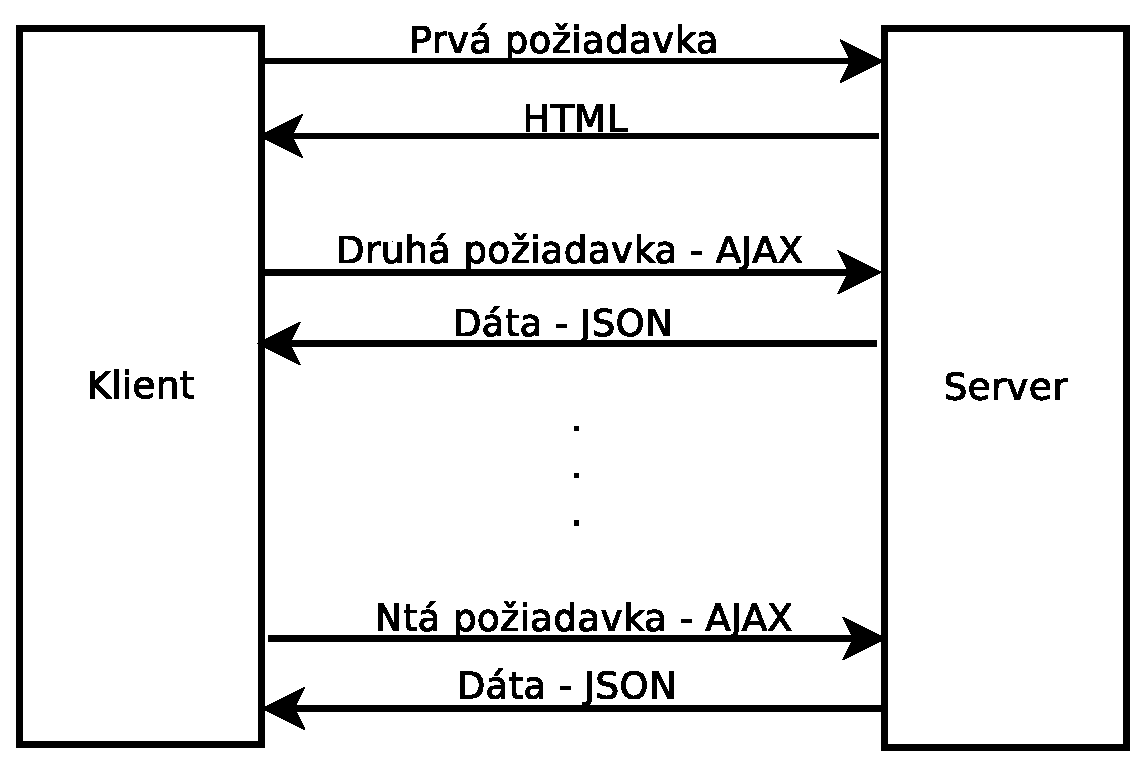
\includegraphics[scale=0.5]{fig/spa.eps}
        \caption{Klient-server komunikácia v Single page aplikácii.}
        \label{fig:spa}
    \end{figure}
    \pagebreak
    \item \textbf{Cordova -} je rámec, ktorý zabalí HTML, CSS a Javascript aplikáciu do natívneho kontaineru, WebView, ktorý vo výsledku vyzerá a chová sa ako bežná natívna aplikácia. Kontainer dokáže pristupovať k funkciám zariadenia vďaka natívnym zásuvným modulom a Javascriptovému aplikačnému rozhraniu. Cordova podporuje celú škálu platforiem od Android, cez iOS, až po Windows Phone. Projekt bol najprv vytvorený firmou Nitobi, ktorá bola v roku 2011 kúpená známou firmou Adobe Systems. Adobe Systems následne uvoľnila kód Cordovy. \cite{DVKuXjtaapUpB12M}
    \begin{figure}[h]
      \centering
      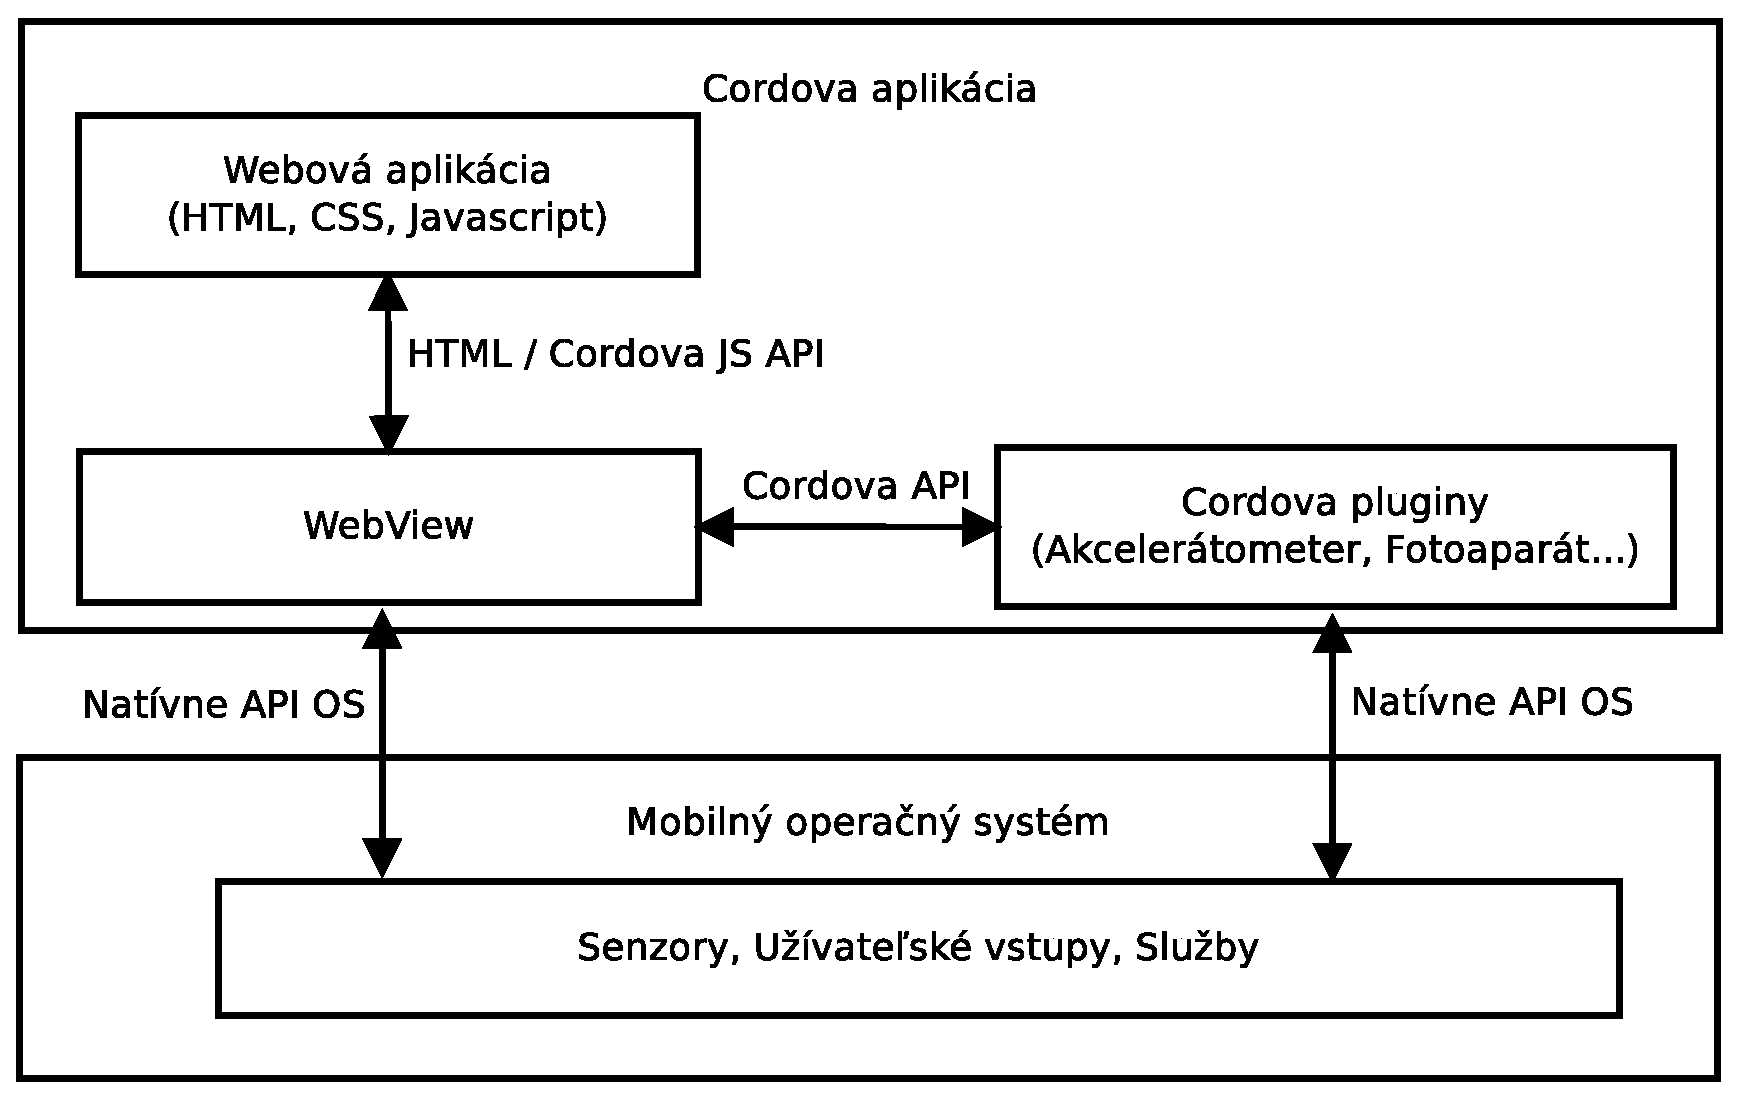
\includegraphics[scale=0.35]{fig/cordova.eps}
      \caption{Architektúra aplikácie vytvorenej pomocou Cordova technológie.}
      \label{fig:cordova}
    \end{figure}
    \item \textbf{Ionic2 -} je kompletné SDK pre vývoj hybridných mobilných aplikácií. Celý aplikačný rámec je postavený na Angular2 a  rozširuje ho o ďalšie komponenty a funkcionalitu typickú pre mobilné zariadenia. Pomocou Cordova zásuvným modulom a ich implementácií v tomto rámci je možné tiež pristupovať k natívnym funkciám zariadenia. \cite{HiUt1XS9KvN1fiB5}
    
    Hybridné mobilné aplikácie sú aplikácie, ktoré na prvý pohľad vypadajú ako natívne aplikácie, avšak ich programovanie prebiehalo väčšinou pomocou webových technológií s následným zabalením pomocou technológie Cordova, alebo inej podobnej. Medzi  najväčšiu výhodu takéhoto prístupu patrí to, že aplikáciu stačí napísať iba raz a potom ju je možné už iba s drobnými zmenami vydávať na rôzne mobilné platformy.\cite{0QSW9GoG0OTJ7FKM}
    \item \textbf{Electron -} je knižnica vyvinutá GitHubom pre tvorbu multiplatformných desktopových aplikácií pomocou webových technológií, ktoré už boli popísané. Electron je ponúkaný pod licenciou MIT a má otvorený kód. Využíva kombináciu technológie Chromium a Node.js, ktoré zabalí spolu s webovou aplikáciou do jednej výslednej aplikácie. Takúto výslednú aplikáciu je možné spúšťať na platforme Windows, Mac a aj Linux. K natívnym funkciám operačného systému je možné pristupovať, tak ako v prípade Cordovy, pomoocu natívnych aplikačných rozhraní. \cite{hBGbGXxiU66nJt51}
    \begin{figure}[h]
      \centering
      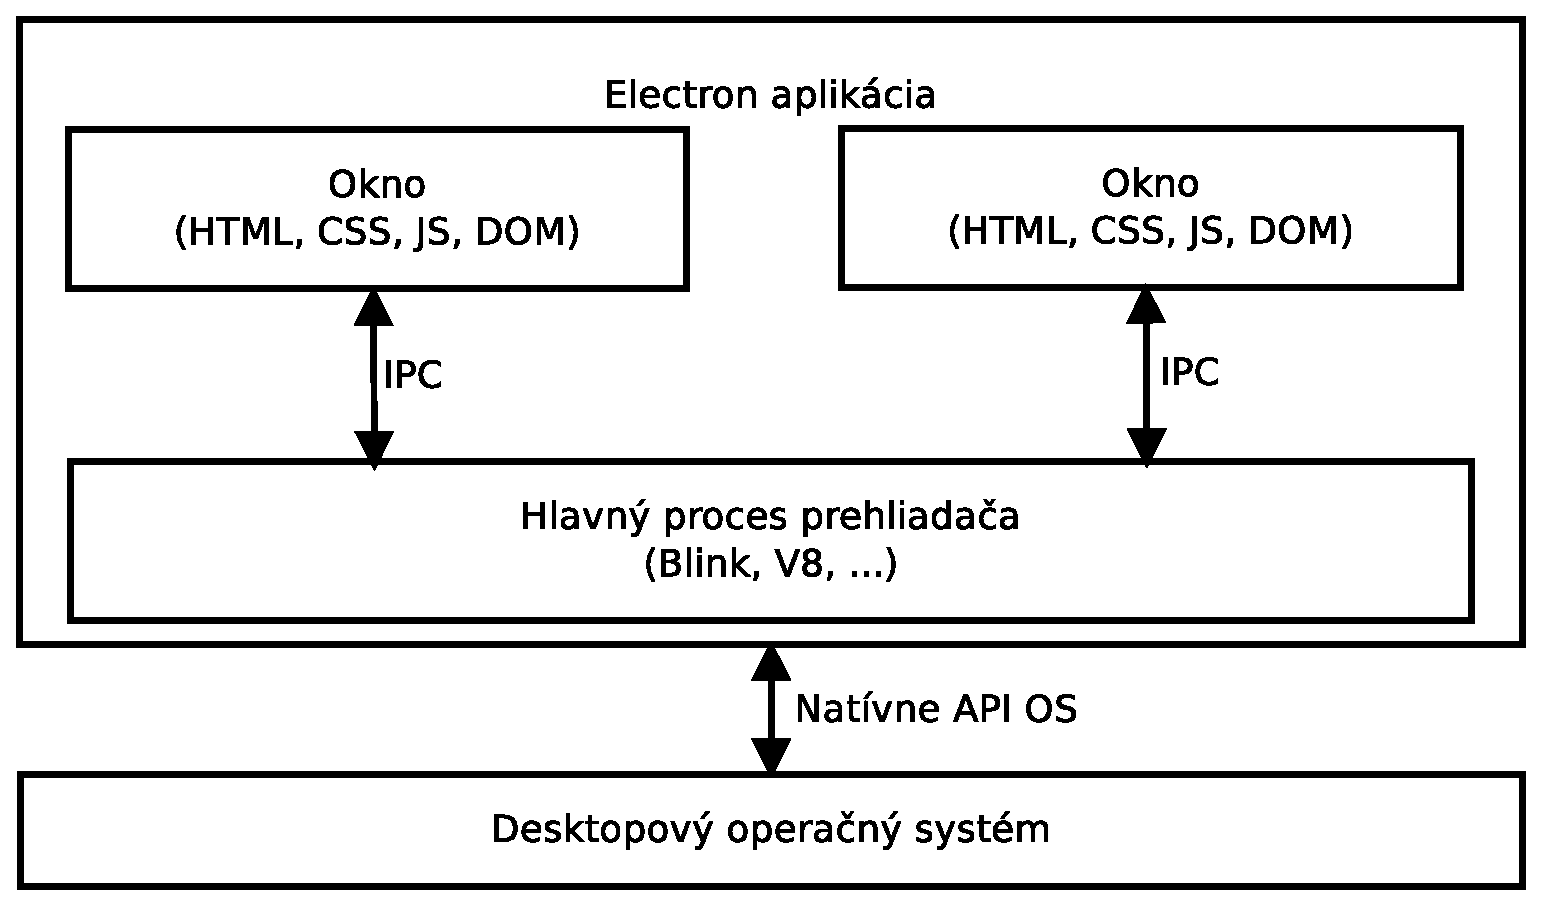
\includegraphics[scale=0.40]{fig/electron.eps}
      \caption{Architektúra aplikácie vytvorenej pomocou Electron rámca.}
      \label{fig:electron}
    \end{figure}
\end{itemize}

\section{Serverová časť - aplikačné rozhranie}
Serverová časť pokrýva všetky operácie, ktoré sa nevykonávajú priamo v zariadení, ale vykonávajú sa vzdialene na strane serveru. Medzi takéto operácie patrí napríklad ukladanie dát do databáze, autentifikácia, autorizácia užívateľa, alebo samotná práca so snímkom chronickej rany. Serverová časť v tejto práci tvorí vzdialené aplikačné rozhranie. Je tvorená pomocou skriptovacieho jazyka Python, za pomoci aplikačného rámca Flask. Flask vo svojom jadre dodržiava princípy REST a je vďaka tomu možné jednoducho navrhnúť plne funkčné RESTful aplikačné rozhranie, s ktorým v tejto práci priamo komunikuje klientská aplikácia. Pre spracovanie obrazu, konkrétne samotných fotiek chronických rán, bola vybraná Python implementácia populárnej knižnice na spracovanie obrazu zvaná OpenCV.
\begin{itemize}
    \item \textbf{REST -} Representational state transfer je súbor niekoľkých prísnych, ale jasne definovaných pravidiel pre návrh architektúry distribuovaného systému, hlavne rozhrania medzi jednotlivými komponentami, poprípade serverovou a klientskou časťou. Základným stavebným kameňom RESTu je zdroj. Zdroj môže byť čokoľvek, napríklad konkrétny objekt v databáze, dokument a podobne. Základným pravidlom je, že každý objekt musí mať svoju URL. Klient nikdy nevidí zdroj priamo, ale vždy iba jeden z jeho obrazov, ktorý je nazývaný reprezentácia. Reprezentácia je strojovo čitateľná reprezentácia aktuálneho stavu zdroja. Môže to byť obrázok, HTML stránka a podobne. Výber reprezentácie môže byť ovplyvnený klientom pomocou riadiacej informácie, alebo serverom na základe klasifikácie klienta. Samotná komunikácia cez REST je bezstavová, čo znamená, že každý požiadavok obsahuje všetky informácie potrebné k jeho vykonaniu. REST definuje 4 základné operácie: POST pre vytváranie, GET pre získavanie, PUT pre zmenu a DELETE pre vymazávanie. \cite{54r2mhdAeuyxzZPp}
    \item \textbf{Python -} je open source objektovo-orientovaný vysokoúrovňový skriptovaci jazyk, ktorý vytvoril Guido van Rossum v rokoch 1985-1990. Kód Pythonu spadá pod licenciu GNU General Public License. Python je interpretovaný a teda nie je nutné programy v ňom napísané prekladať. Programy sú namiesto prekladu priamo vykonávané interpreterom. Okrem toho je taktiež interaktívny. To znamená, že užívateľ môže priamo interagovať s interpreterom a písať programy aj týmto spôsobom. Ďalšou nespornou výhodou Pythonu je to, že je rozšíriteľný a nízko-úrovňové moduly sa dajú písať v programovacom jazyku C. Vďaka tomu môže byť dosiahnuté lepšej efektivity. \cite{CCnsn576LIGBCH2C}
    
    Python bol zvolený najmä kvôli tomu, že je pomerne rozšírený, bežne sa používa na serverovú časť webových informačných systémov, má na výber z veľkého množstva intuitívnych aplikačných rámcov, dobre si rozumie s relačnými, ale aj s NoQSL databázami a v neposlednom rade je preň dostupná implementácia OpenCV.
    \item \textbf{Flask -} je aplikačný mini rámec, ktorý je napísaný v programovacom jazyku Python. Slúži pre vývoj webových aplikácií, alebo vo všeobecnosti serverových častí informačných systémov, poprípade aplikačných rozhraní. V základe má k dispozícií iba funkcie s prácou pre URL, HTTP a šablónami. Z toho plynie, že je jednoduchý na osvojenie a pre účely tejto práce úplne postačuje. \cite{YNlrXY2RKWca3gk8}
    \item \textbf{OpenCV -} je knižnica počítačového videnia. Je napísaná v jazyku C a C++ a je možné ju použiť na všetkých bežných aktuálnych platformách. Rozhranie je dostupné pre Python, Java, Ruby a ostatné bežné programovacie jazyky. OpenCV bolo navrhnuté pre výpočtovú efektivitu so silným dôrazom na aplikácie bežiace v reálnom čase. Optimalizácie knižnice boli vykonávané na všetkých úrovniach, od algoritmov až po viac jadrové inštrukcie procesorov. Hlavným cieľom je ponúknuť jednoduchú infraštruktúru počítačového videnia, ktorá by pomáhala ľuďom tvoriť zložitejšie aplikácie oveľa rýchlejšie a jednoduchšie. Samotná knižnica obsahuje viac ako 500 funkcií, pokrývajúce rôzne odvetvia vedy. OpenCV v sebe obsahuje okrem svojej samotnej implementácie aj pod-knižnice pre strojové učenie. keďže počítačové videnie a strojové učenie spolu úzko súvisia. Pod-knižnice sa z veľkej časti orientujú na rozpoznávanie vzorov a rozdeľovanie do zhlukov. \cite{Bradskic2008}
\end{itemize}

\section{Databázová časť}
Pre uchovanie dát na strane serveru bola zvolená možnosť uloženia do databáze. Táto možnosť bola zvolená kvôli tomu, že manipulácia s dátami je pomerne rýchla, keďže sa do pamäte neukladá celá databáza, ale iba jej požadovaná časť. Okrem toho, pre získanie dát sa dá použiť pokročilejší dotazovací jazyk a je podporovaný prístup viacerých užívateľov súčasne. 

Ako databáza bol zvolený typický zástupca NoSQL databáz menom MongoDB, ktorý je vyvíjaný MongoDB industries a má otvorený zdrojový kód. Dáta ukladá v štruktúre podobnej JSON dokumentom, a to v štruktúre Binary JSON, ktorý samotný JSON obohacuje o ďalšie typy. Súvisiace informácie sú uložené spolu pre rýchly dotazovací prístup pomocou MongoDB dotazovacieho jazyka. Používa dynamické schémy, to znamená, že záznamy nemajú pevne danú štruktúru a v priebehu sa táto štruktúra môže meniť. Pomocou tohoto dátového modelu je možné reprezentovať hierarchické vzťahy a ukladať polia a iné komplexnejšie dátové štruktúry. MongoDB dbá na to, aby bola zabezpečená vysoká dostupnosť a škálovateľnosť. Nespornou výhodou NoSQL a konkrétne MongoDB oproti Mysql je, že vývoj aplikácie s MongoDB je jednoduchší, keďže sa dokumenty v databáze prirodzene mapujú do moderných objektovo orientovaných jazykov a odpadá tak objektovo relačné mapovanie objektov. Obrovskou výhodou oproti napríklad MySQL je už spomínaná škálovateľnosť. Samotné MongoDB vyžaduje pre svoje fungovanie iba adresár na uloženie dát a teda môže byť ľahko distribuované spolu s programom. \cite{9egOMsyThyK0MyF2}
\begin{lstlisting}[caption={Ukážka štruktúry NoSQL MongoDB databáze.},captionpos=b]
[
    item1ID: {
	    name: 'MongoDB',
	    description: 'NoSQL'
    },
    item2ID: {
	    name: 'MySQL',
	    description: 'Relational'
    }
]
\end{lstlisting}

\chapter{Analýza a návrh riešenia}
TODO
